%%%%%%%%%%%%%%%%%%%%%%%%%%%%%%%%%%%%%%%%%%%%%%%%%%%%%%%%%%%%%%%%%%
%%%%%%%% ICML 2012 EXAMPLE LATEX SUBMISSION FILE %%%%%%%%%%%%%%%%%
%%%%%%%%%%%%%%%%%%%%%%%%%%%%%%%%%%%%%%%%%%%%%%%%%%%%%%%%%%%%%%%%%%

% Use the following line _only_ if you're still using LaTeX 2.09.
%\documentstyle[icml2012,epsf,natbib]{article}
% If you rely on Latex2e packages, like most moden people use this:
\documentclass{article}

% For figures
\usepackage{graphicx} % more modern
%\usepackage{epsfig} % less modern
\usepackage{subfigure} 

% For citations
\usepackage{natbib}

% For algorithms
\usepackage{algorithm}
\usepackage{algorithmic}

% As of 2011, we use the hyperref package to produce hyperlinks in the
% resulting PDF.  If this breaks your system, please commend out the
% following usepackage line and replace \usepackage{icml2012} with
% \usepackage[nohyperref]{icml2012} above.
\usepackage{hyperref}

% Packages hyperref and algorithmic misbehave sometimes.  We can fix
% this with the following command.
\newcommand{\theHalgorithm}{\arabic{algorithm}}

% Employ the following version of the ``usepackage'' statement for
% submitting the draft version of the paper for review.  This will set
% the note in the first column to ``Under review.  Do not distribute.''
%\usepackage{icml2012} 
% Employ this version of the ``usepackage'' statement after the paper has
% been accepted, when creating the final version.  This will set the
% note in the first column to ``Appearing in''
 \usepackage[accepted]{icml2012}


% The \icmltitle you define below is probably too long as a header.
% Therefore, a short form for the running title is supplied here:
\icmltitlerunning{Submission and Formatting Instructions for ICML 2012}

\begin{document} 

\twocolumn[
\icmltitle{2D Cancer Visualization by Dimensionality Reduction of Immune System Cellular Protein Data}

% It is OKAY to include author information, even for blind
% submissions: the style file will automatically remove it for you
% unless you've provided the [accepted] option to the icml2012
% package.
\icmlauthor{Your Name}{email@yourdomain.edu}
\icmladdress{Your Fantastic Institute,
            314159 Pi St., Palo Alto, CA 94306 USA}
\icmlauthor{Your CoAuthor's Name}{email@coauthordomain.edu}
\icmladdress{Their Fantastic Institute,
            27182 Exp St., Toronto, ON M6H 2T1 CANADA}

% You may provide any keywords that you 
% find helpful for describing your paper; these are used to populate 
% the "keywords" metadata in the PDF but will not be shown in the document
\icmlkeywords{boring formatting information, machine learning, ICML}

\vskip 0.3in
]

\begin{abstract} 
ICML 2012 full paper submissions are due February 24, 2012. Reviewing will
be blind to the identities of the authors, and therefore identifying
information must not appear in any way in papers submitted for review. Submissions must be in PDF, 8 page length limit.
\end{abstract} 

\section{Electronic Submission}
\label{submission}

As in the past few years, ICML will rely exclusively on
electronic formats for submission and review. 


\subsection{Templates for Papers}

Electronic templates for producing papers for submission are available
for \LaTeX\/ and Microsoft Word. Templates are accessible on the World
Wide Web at:\\
\textbf{\texttt{http://icml.cc/2012/}}

\noindent
Send questions about these electronic templates to
\texttt{program@icml.cc}.

The formatting instructions below will be enforced for initial submissions and camera-ready copies. 
\begin{itemize}
\item The maximum paper length is 8 pages.
\item Do not alter the style template; in particular, do not compress the paper format by reducing the vertical spaces.
\item Do not include author information or acknowledgments in your
  initial submission. 
\item Place figure captions {\em under} the figure (and omit titles from
  inside the graphic file itself).  Place table captions {\em over}
  the table.
\item References must include page numbers whenever possible and be as
  complete as possible.  Place multiple citations in chronological order.  
\end{itemize}
Please see below for details on each of these items.

\subsection{Submitting Papers}

Submission to ICML 2012 will be entirely electronic, via a web site
(not email).  The URL and information about the submission process
are available on the conference web site at

\textbf{\texttt{http://icml.cc/2012/}}

{\bf Paper Deadline:} The deadline for paper submission to ICML 2012
is Friday, February 24, 2012, at 23:59 Universal Time (3:59 Pacific Daylight Time).  If your full
submission does not reach us by this date, it will not be considered
for publication. There is no separate abstract submission.

{\bf Anonymous Submission:} To facilitate blind review, no identifying
author information should appear on the title page or in the paper
itself.  Section~\ref{author info} will explain the details of how to
format this.

{\bf Simultaneous Submission:} ICML will not accept any paper which,
at the time of submission, is under review for another conference or
has already been published. This policy also applies to papers that
overlap substantially in technical content with conference papers
under review or previously published. ICML submissions must not be
submitted to other conferences during ICML's review period. Authors
may submit to ICML substantially different versions of journal papers
that are currently under review by the journal, but not yet accepted
at the time of submission. Informal publications, such as technical
reports or papers in workshop proceedings which do not appear in
print, do not fall under these restrictions.

\medskip

To ensure our ability to print submissions, authors must provide their
manuscripts in \textbf{PDF} format.  Furthermore, please make sure
that files contain only Type-1 fonts (e.g.,~using the program {\tt
  pdffonts} in linux or using File/DocumentProperties/Fonts in
Acrobat).  Other fonts (like Type-3) might come from graphics files
imported into the document.

Authors using \textbf{Word} must convert their document to PDF.  Most
of the latest versions of Word have the facility to do this
automatically.  Submissions will not be accepted in Word format or any
format other than PDF. Really. We're not joking. Don't send Word.

Those who use \textbf{\LaTeX} to format their accepted papers need to
pay close attention to the typefaces used.  Specifically, when
producing the PDF by first converting the dvi output of \LaTeX\ to Postscript
the default behavior is to use non-scalable Type-3 PostScript bitmap
fonts to represent the standard \LaTeX\ fonts. The resulting document
is difficult to read in electronic form; the type appears fuzzy. To
avoid this problem, dvips must be instructed to use an alternative
font map.  This can be achieved with
something like the following commands:\\[0.5em]
{\bf dvips -Ppdf -tletter -G0 -o paper.ps paper.dvi}\\
{\bf ps2pdf paper.ps}\\[0.5em]
Note that it is a zero following the ``-G''.  This tells dvips to use
the config.pdf file (and this file refers to a better font mapping).

Another alternative is to use the \textbf{pdflatex} program instead of
straight \LaTeX. This program avoids the Type-3 font problem, however
you must ensure that all of the fonts are embedded (use {\tt
pdffonts}). If they are not, you need to configure pdflatex to use a
font map file that specifies that the fonts be embedded. Also you
should ensure that images are not downsampled or otherwise compressed
in a lossy way.

Note that the 2012 style files use the {\tt hyperref} package to
make clickable links in documents.  If this causes problems for you,
add {\tt nohyperref} as one of the options to the {\tt icml2012}
usepackage statement.

\subsection{Reacting to Reviews}
We will continue the ICML tradition in which the authors are given the
option of providing a short reaction to the initial reviews. These
reactions will be taken into account in the discussion among the
reviewers and area chairs.

\subsection{Submitting Final Camera-Ready Copy}

The final versions of papers accepted for publication should follow the
same format and naming convention as initial submissions, except of
course that the normal author information (names and affiliations)
should be given.  See Section~\ref{final author} for details of how to
format this.

The footnote, ``Preliminary work.  Under review by the International
Conference on Machine Learning (ICML).  Do not distribute.'' must be
modified to ``Appearing in \textit{Proceedings of the
$\mathit{29}^{th}$ International Conference on Machine Learning},
Edinburgh, Scotland, UK, 2012.  Copyright 2012 by the author(s)/owner(s).''

For those using the \textbf{\LaTeX} style file, simply change
$\mathtt{\backslash usepackage\{icml2012\}}$ to 

\verb|\usepackage[accepted]{icml2012}|

\noindent
Authors using \textbf{Word} must edit the
footnote on the first page of the document themselves.

Camera-ready copies should have the title of the paper as running head
on each page except the first one.  The running title consists of a
single line centered above a horizontal rule which is $1$ point thick.
The running head should be centered, bold and in $9$ point type.  The
rule should be $10$ points above the main text.  For those using the
\textbf{\LaTeX} style file, the original title is automatically set as running
head using the {\tt fancyhdr} package which is included in the ICML
2012 style file package.  In case that the original title exceeds the
size restrictions, a shorter form can be supplied by using

\verb|\icmltitlerunning{...}|

just before $\mathtt{\backslash begin\{document\}}$.
Authors using \textbf{Word} must edit the header of the document themselves.

\section{Format of the Paper} 
 
All submissions must follow the same format to ensure the printer can
reproduce them without problems and to let readers more easily find
the information that they desire.

\subsection{Length and Dimensions}

Papers must not exceed eight (8) pages, including all figures, tables,
references, and appendices. Any submission that exceeds this page
limit or that diverges significantly from the format specified herein
will be rejected without review.

The text of the paper should be formatted in two columns, with an
overall width of 6.75 inches, height of 9.0 inches, and 0.25 inches
between the columns. The left margin should be 0.75 inches and the top
margin 1.0 inch (2.54~cm). The right and bottom margins will depend on
whether you print on US letter or A4 paper, but all final versions
must be produced for US letter size.

The paper body should be set in 10~point type with a vertical spacing
of 11~points. Please use Times Roman typeface throughout the text.

\subsection{Title}

The paper title should be set in 14~point bold type and centered
between two horizontal rules that are 1~point thick, with 1.0~inch
between the top rule and the top edge of the page. Capitalize the
first letter of content words and put the rest of the title in lower
case.

\subsection{Author Information for Submission}
\label{author info}

To facilitate blind review, author information must not appear.  If
you are using \LaTeX\/ and the \texttt{icml2012.sty} file, you may use
\verb+\icmlauthor{...}+ to specify authors.  The author information
will simply not be printed until {\tt accepted} is an argument to the
style file. Submissions that include the author information will not
be reviewed.

\subsubsection{Self-Citations}

If your are citing published papers for which you are an author, refer
to yourself in the third person. In particular, do not use phrases
that reveal your identity (e.g., ``in previous work \cite{langley00}, we 
have shown \ldots'').

Do not anonymize citations in the reference section by removing or
blacking out author names. The only exception are manuscripts that are
not yet published (e.g. under submission). If you choose to refer to
such unpublished manuscripts \cite{anonymous}, anonymized copies have to be submitted
as Supplementary Material via CMT. However, keep in mind that an ICML
paper should be self contained and should contain sufficient detail
for the reviewers to evaluate the work. In particular, reviewers are
not required to look a the Supplementary Material when writing their
review.

\subsubsection{Camera-Ready Author Information}
\label{final author}

If a paper is accepted, a final camera-ready copy must be prepared.
%
For camera-ready papers, author information should start 0.3~inches
below the bottom rule surrounding the title. The authors' names should
appear in 10~point bold type, electronic mail addresses in 10~point
small capitals, and physical addresses in ordinary 10~point type.
Each author's name should be flush left, whereas the email address
should be flush right on the same line. The author's physical address
should appear flush left on the ensuing line, on a single line if
possible. If successive authors have the same affiliation, then give
their physical address only once.

A sample file (in PDF) with author names is included in the ICML2012 style file package.

\subsection{Abstract}

The paper abstract should begin in the left column, 0.4~inches below
the final address. The heading `Abstract' should be centered, bold,
and in 11~point type. The abstract body should use 10~point type, with
a vertical spacing of 11~points, and should be indented 0.25~inches
more than normal on left-hand and right-hand margins. Insert
0.4~inches of blank space after the body. Keep your abstract brief and self-contained,
limiting it to one paragraph and no more than six or seven sentences.

\subsection{Partitioning the Text} 

You should organize your paper into sections and paragraphs to help
readers place a structure on the material and understand its
contributions.

\subsubsection{Sections and Subsections}

Section headings should be numbered, flush left, and set in 11~pt bold
type with the content words capitalized. Leave 0.25~inches of space
before the heading and 0.15~inches after the heading.

Similarly, subsection headings should be numbered, flush left, and set
in 10~pt bold type with the content words capitalized. Leave
0.2~inches of space before the heading and 0.13~inches afterward.

Finally, subsubsection headings should be numbered, flush left, and
set in 10~pt small caps with the content words capitalized. Leave
0.18~inches of space before the heading and 0.1~inches after the
heading. 

Please use no more than three levels of headings.

\subsubsection{Paragraphs and Footnotes}

Within each section or subsection, you should further partition the
paper into paragraphs. Do not indent the first line of a given
paragraph, but insert a blank line between succeeding ones.
 
You can use footnotes\footnote{For the sake of readability, footnotes
should be complete sentences.} to provide readers with additional
information about a topic without interrupting the flow of the paper. 
Indicate footnotes with a number in the text where the point is most
relevant. Place the footnote in 9~point type at the bottom of the
column in which it appears. Precede the first footnote in a column
with a horizontal rule of 0.8~inches.\footnote{Multiple footnotes can
appear in each column, in the same order as they appear in the text,
but spread them across columns and pages if possible.}

\begin{figure}[ht]
\vskip 0.2in
\begin{center}
\centerline{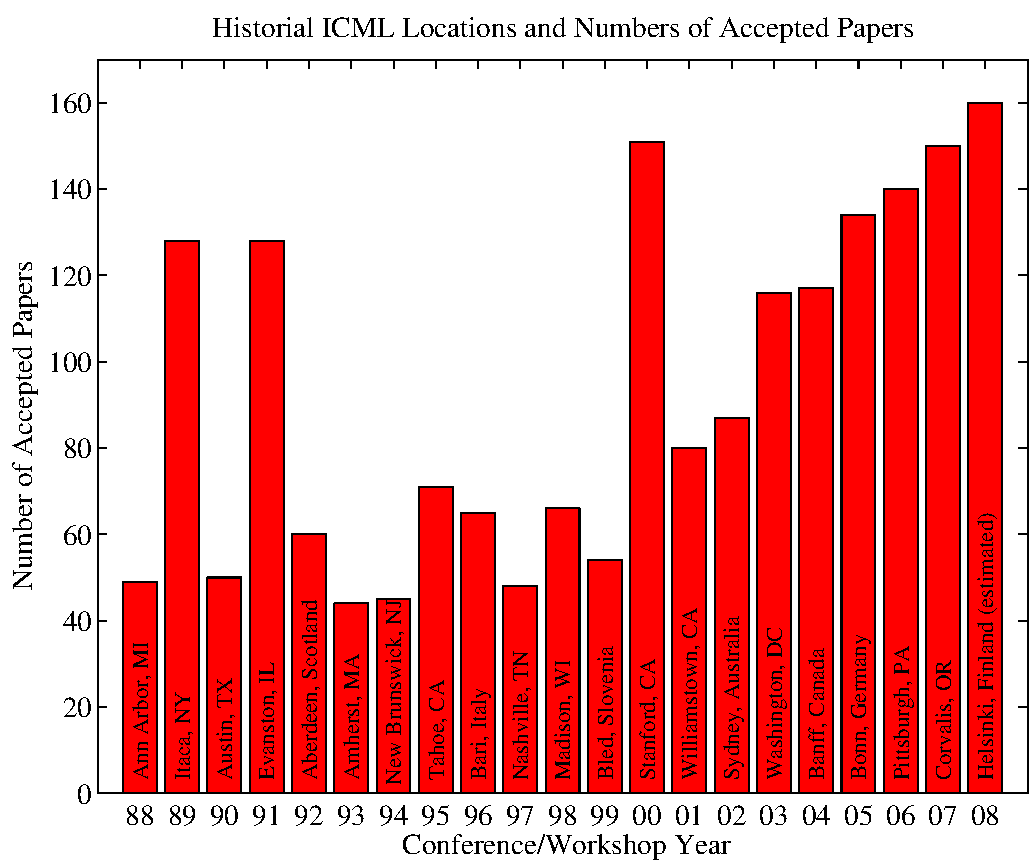
\includegraphics[width=\columnwidth]{icml_numpapers}}
\caption{Historical locations and number of accepted papers for International
  Machine Learning Conferences (ICML 1993 -- ICML 2008) and
  International Workshops on Machine Learning (ML 1988 -- ML
  1992). At the time this figure was produced, the number of
  accepted papers for ICML 2008 was unknown and instead estimated.}
\label{icml-historical}
\end{center}
\vskip -0.2in
\end{figure} 

\subsection{Figures}
 
You may want to include figures in the paper to help readers visualize
your approach and your results. Such artwork should be centered,
legible, and separated from the text. Lines should be dark and at
least 0.5~points thick for purposes of reproduction, and text should
not appear on a gray background.

Label all distinct components of each figure. If the figure takes the
form of a graph, then give a name for each axis and include a legend
that briefly describes each curve. Do not include a title inside the
figure; instead, the caption should serve this function.

Number figures sequentially, placing the figure number and caption
{\it after\/} the graphics, with at least 0.1~inches of space before
the caption and 0.1~inches after it, as in
Figure~\ref{icml-historical}.  The figure caption should be set in
9~point type and centered unless it runs two or more lines, in which
case it should be flush left.  You may float figures to the top or
bottom of a column, and you may set wide figures across both columns
(use the environment {\tt figure*} in \LaTeX), but always place
two-column figures at the top or bottom of the page.

\subsection{Algorithms}

If you are using \LaTeX, please use the ``algorithm'' and ``algorithmic'' 
environments to format pseudocode. These require 
the corresponding stylefiles, algorithm.sty and 
algorithmic.sty, which are supplied with this package. 
Algorithm~\ref{alg:example} shows an example. 

\begin{algorithm}[tb]
   \caption{Bubble Sort}
   \label{alg:example}
\begin{algorithmic}
   \STATE {\bfseries Input:} data $x_i$, size $m$
   \REPEAT
   \STATE Initialize $noChange = true$.
   \FOR{$i=1$ {\bfseries to} $m-1$}
   \IF{$x_i > x_{i+1}$} 
   \STATE Swap $x_i$ and $x_{i+1}$
   \STATE $noChange = false$
   \ENDIF
   \ENDFOR
   \UNTIL{$noChange$ is $true$}
\end{algorithmic}
\end{algorithm}
 
\subsection{Tables} 
 
You may also want to include tables that summarize material. Like 
figures, these should be centered, legible, and numbered consecutively. 
However, place the title {\it above\/} the table with at least 
0.1~inches of space before the title and the same after it, as in 
Table~\ref{sample-table}. The table title should be set in 9~point 
type and centered unless it runs two or more lines, in which case it
should be flush left.

% Note use of \abovespace and \belowspace to get reasonable spacing 
% above and below tabular lines. 

\begin{table}[t]
\caption{Classification accuracies for naive Bayes and flexible 
Bayes on various data sets.}
\label{sample-table}
\vskip 0.15in
\begin{center}
\begin{small}
\begin{sc}
\begin{tabular}{lcccr}
\hline
\abovespace\belowspace
Data set & Naive & Flexible & Better? \\
\hline
\abovespace
Breast    & 95.9$\pm$ 0.2& 96.7$\pm$ 0.2& $\surd$ \\
Cleveland & 83.3$\pm$ 0.6& 80.0$\pm$ 0.6& $\times$\\
Glass2    & 61.9$\pm$ 1.4& 83.8$\pm$ 0.7& $\surd$ \\
Credit    & 74.8$\pm$ 0.5& 78.3$\pm$ 0.6&         \\
Horse     & 73.3$\pm$ 0.9& 69.7$\pm$ 1.0& $\times$\\
Meta      & 67.1$\pm$ 0.6& 76.5$\pm$ 0.5& $\surd$ \\
Pima      & 75.1$\pm$ 0.6& 73.9$\pm$ 0.5&         \\
\belowspace
Vehicle   & 44.9$\pm$ 0.6& 61.5$\pm$ 0.4& $\surd$ \\
\hline
\end{tabular}
\end{sc}
\end{small}
\end{center}
\vskip -0.1in
\end{table}

Tables contain textual material that can be typeset, as contrasted 
with figures, which contain graphical material that must be drawn. 
Specify the contents of each row and column in the table's topmost
row. Again, you may float tables to a column's top or bottom, and set
wide tables across both columns, but place two-column tables at the
top or bottom of the page.
 
\subsection{Citations and References} 

Please use APA reference format regardless of your formatter
or word processor. If you rely on the \LaTeX\/ bibliographic 
facility, use {\tt natbib.sty} and {\tt icml2012.bst} 
included in the style-file package to obtain this format.

Citations within the text should include the authors' last names and
year. If the authors' names are included in the sentence, place only
the year in parentheses, for example when referencing Arthur Samuel's
pioneering work \yrcite{Samuel59}. Otherwise place the entire
reference in parentheses with the authors and year separated by a
comma \cite{Samuel59}. List multiple references separated by
semicolons \cite{kearns89,Samuel59,mitchell80}. Use the `et~al.'
construct only for citations with three or more authors or after
listing all authors to a publication in an earlier reference \cite{MachineLearningI}.

Authors should cite their own work in the third person
in the initial version of their paper submitted for blind review.
Please refer to Section~\ref{author info} for detailed instructions on how to
cite your own papers.

Use an unnumbered first-level section heading for the references, and 
use a hanging indent style, with the first line of the reference flush
against the left margin and subsequent lines indented by 10 points. 
The references at the end of this document give examples for journal
articles \cite{Samuel59}, conference publications \cite{langley00}, book chapters \cite{Newell81}, books \cite{DudaHart2nd}, edited volumes \cite{MachineLearningI}, 
technical reports \cite{mitchell80}, and dissertations \cite{kearns89}. 

Alphabetize references by the surnames of the first authors, with
single author entries preceding multiple author entries. Order
references for the same authors by year of publication, with the
earliest first. Make sure that each reference includes all relevant
information (e.g., page numbers).

\subsection{Software and Data}

We strongly encourage the publication of software and data with the
camera-ready version of the paper whenever appropriate.  This can be
done by including a URL in the camera-ready copy.  However, do not
include URLs that reveal your institution or identity in your
submission for review.  Instead, provide an anonymous URL or upload
the material as ``Supplementary Material'' into the CMT reviewing
system.  Note that reviewers are not required to look a this material
when writing their review.


% Acknowledgements should only appear in the accepted version. 
\section*{Acknowledgments} 
 
\textbf{Do not} include acknowledgements in the initial version of
the paper submitted for blind review.

If a paper is accepted, the final camera-ready version can (and
probably should) include acknowledgements. In this case, please
place such acknowledgements in an unnumbered section at the
end of the paper. Typically, this will include thanks to reviewers
who gave useful comments, to colleagues who contributed to the ideas, 
and to funding agencies and corporate sponsors that provided financial 
support.  


% In the unusual situation where you want a paper to appear in the
% references without citing it in the main text, use \nocite
\nocite{langley00}

\bibliography{example_paper}
\bibliographystyle{natbib}
%\bibliographystyle{icml2012}

\end{document} 


% This document was modified from the file originally made available by
% Pat Langley and Andrea Danyluk for ICML-2K. This version was
% created by Lise Getoor and Tobias Scheffer, it was slightly modified  
% from the 2010 version by Thorsten Joachims & Johannes Fuernkranz, 
% slightly modified from the 2009 version by Kiri Wagstaff and 
% Sam Roweis's 2008 version, which is slightly modified from 
% Prasad Tadepalli's 2007 version which is a lightly 
% changed version of the previous year's version by Andrew Moore, 
% which was in turn edited from those of Kristian Kersting and 
% Codrina Lauth. Alex Smola contributed to the algorithmic style files.  


